%xelatex
\documentclass{article}
\usepackage[margin=0.6in]{geometry}
\usepackage{xltxtra}
\usepackage{xgreek}
\usepackage{listings}
\setmainfont[Mapping=tex-text]{Kerkis}
\usepackage[colorlinks=true,linkcolor=black,urlcolor=blue]{hyperref}
\title{Παράλληλη επεξεργασία}
\author{Μπαντολας Πέτρος 5028\\Σειμένης Σπύρος 5070\\Καλλιβωκάς Δημήτριος 4993}

\begin{document}
\maketitle
\section{Ανάλυση σειριακής έκδοσης}
Η συμπεριφορά της σειριακής εκδοσης έγινε με την χρήση του εργαλείου scalasca.
\begin{center}
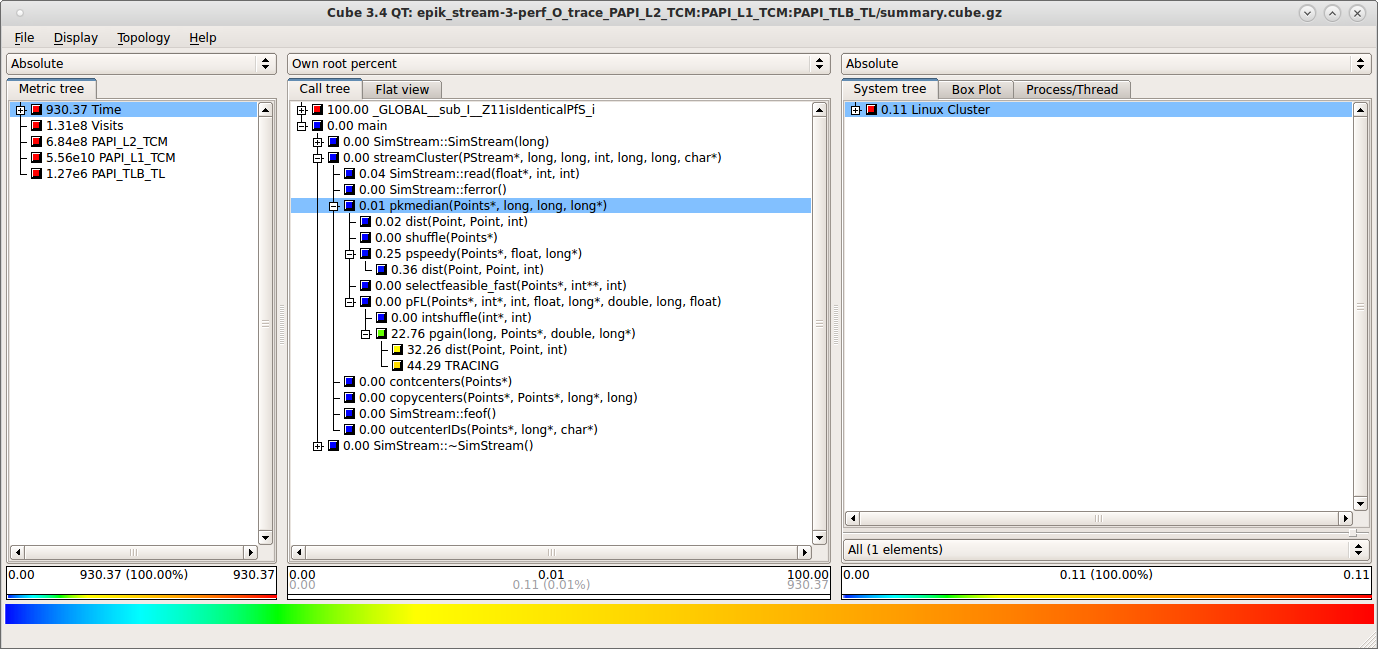
\includegraphics[scale=0.5]{../scrshots/time.png}
\end{center} 
Όπως φαινεται και στην εικόνα, οι συναρτήσεις με τον μεγαλύτερο χρόνο εκτέλεσης ειναι η pspeedy και η pgain.\\
Συγκεκριμένα ο μεγαλύτερος χρόνος και των δύο είναι κατα τις κλήσεις τους στην συνάρτηση dist.
\subsection{pgain}
Παρακάτω φαίνονται τα L1, L2, TLB cache misses της σειριακής έκδοσης όπου επι το πλείστον οφείλονται στην pgain.
\begin{center}
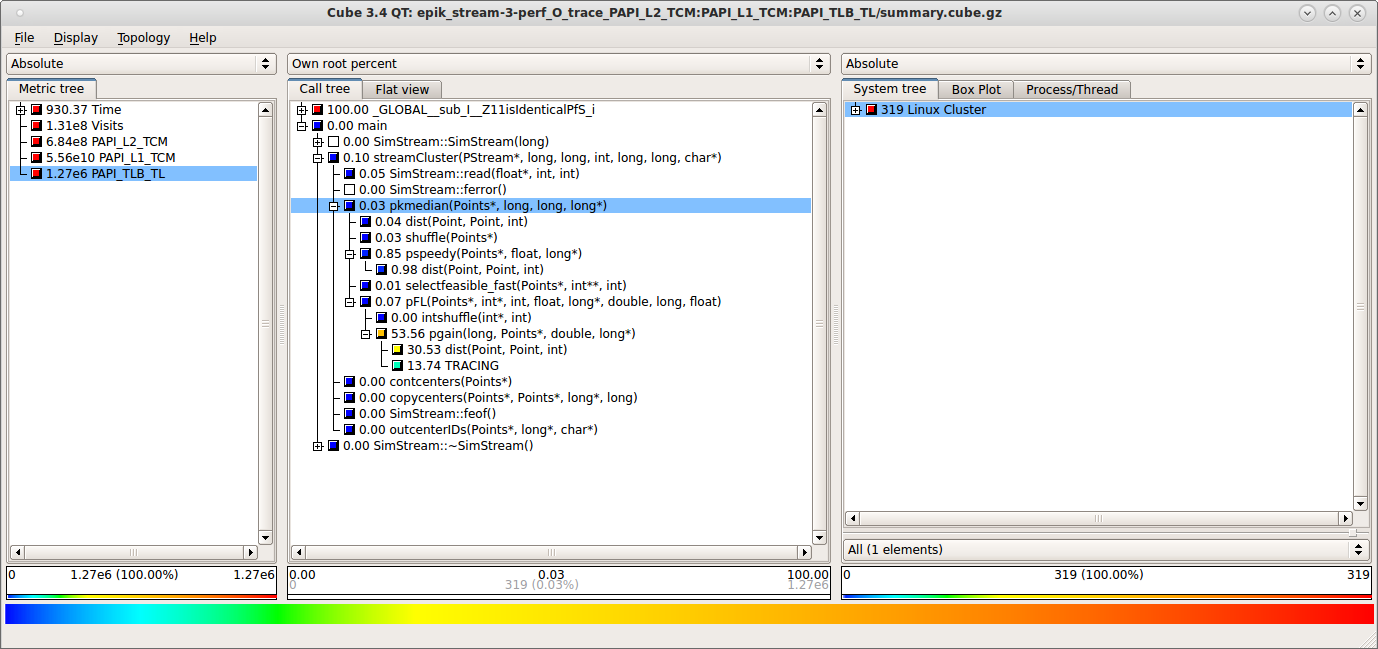
\includegraphics[scale=0.4]{../scrshots/tlb.png}
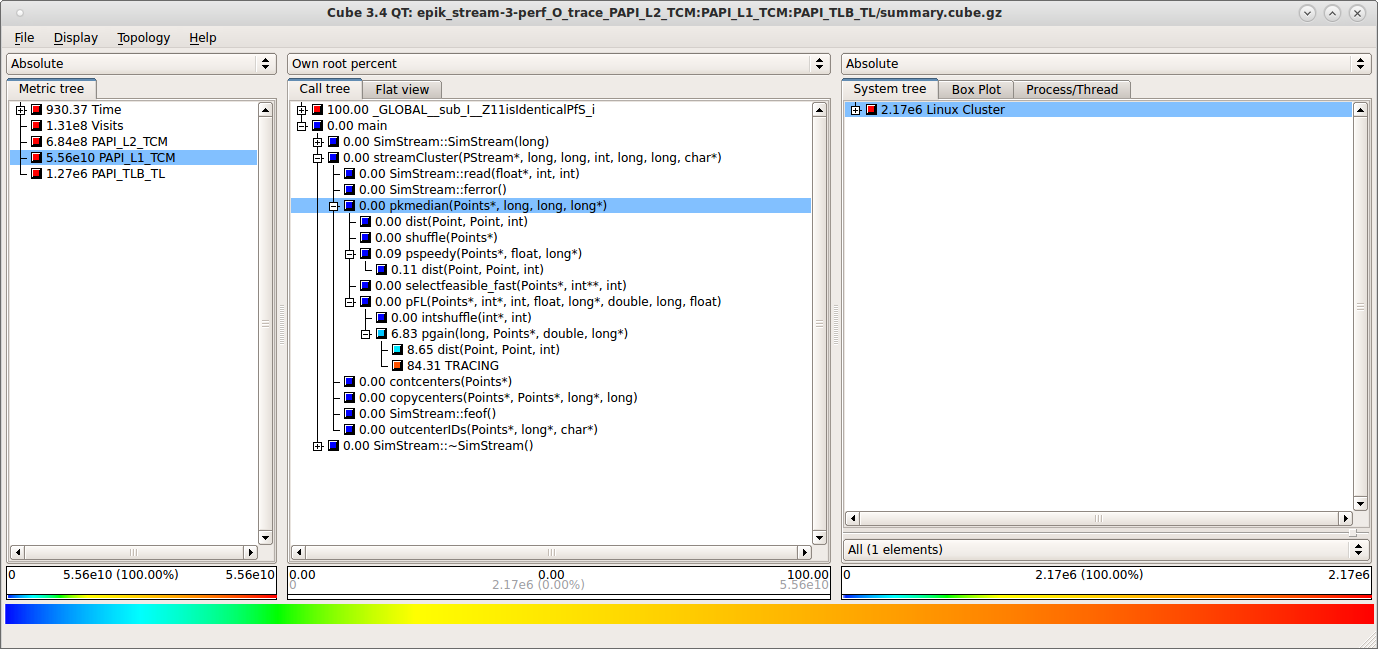
\includegraphics[scale=0.4]{../scrshots/l1.png}
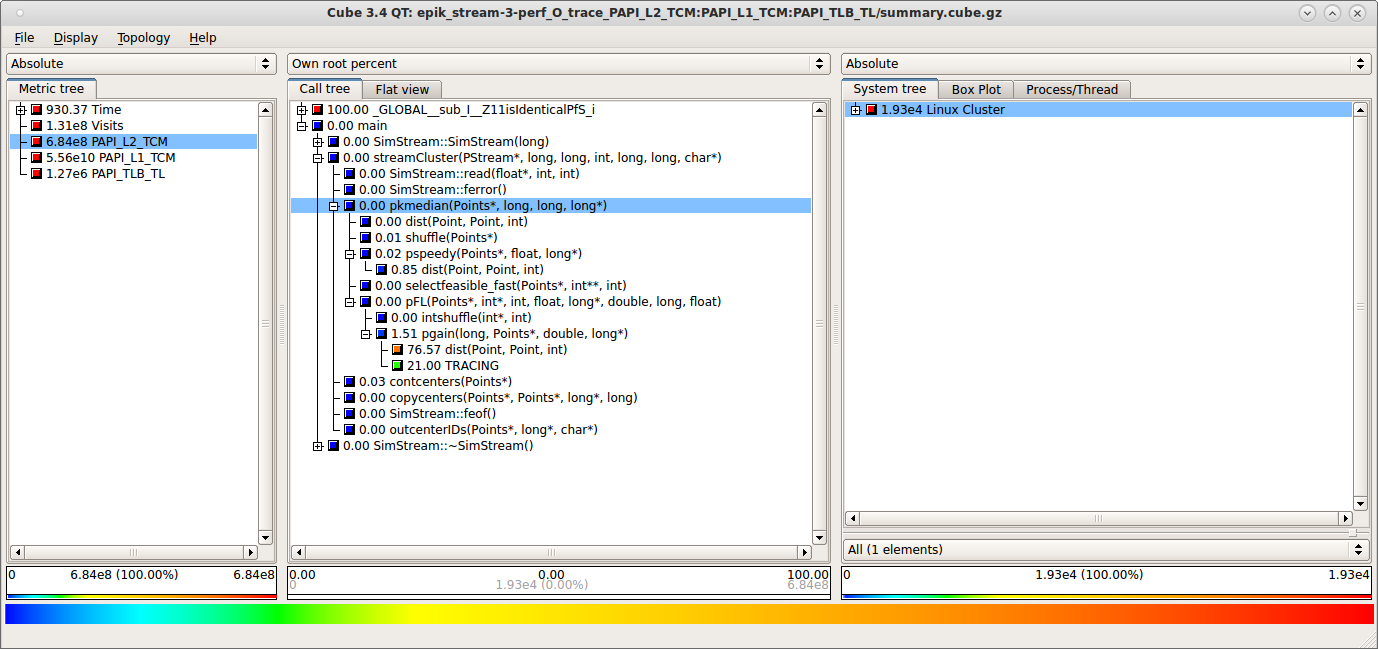
\includegraphics[scale=0.4]{../scrshots/l2.png}
\end{center} 
Συμπεραίνουμε οτι οι περιοχές που προκαλούν καθυστέρηση είναι αυτές που υπολογίζουν κατ' επανάληψη για όλα τα σημεία την απόσταση τους(dist). Αυτό γίνεται για ολα τα σημεία άρα για μεγάλο αριθμό σημείων αυξάνεται και η πολυπλοκοτητα του προγράμματος. Επίσης η δομή που αποθηκεύει τα σημεία δεσμεύεται στην αρχή του προγράμματος στο heap μεσω malloc που δεν εγγυάται ότι οι διευθύνσεις φυσικής μνήμης θα είναι γειτονικες μεταξυ τους. Η πολλαπλή προσπέλαση όλων των σημείων σειριακά οδηγεί στα πολλαπλά cache misses. Έτσι η παραλληλοποίηση με openmp βελτιστοποιεί τους υπολογισμούς μειώνοντας τα cache misses.

\section{Παραλληλοποίηση}
\subsection{Με χρήση OpenMP}
Σύμφωνα με την προηγούμενη ανάλυση, τα σημεία όπου χρειάζεται χρονοβελτίωση είναι κυρίως οι κλήσεις της \texttt{dist} μέσα στις συναρτήσεις \texttt{pgain} και \texttt{pspeedy}.

Δύο είναι τα σημεία μέσα στην \texttt{pgain} όπου καλείται σε βρόχο \texttt{for} η \texttt{dist}. Εισάγοντας εκεί εντολές \texttt{OpenMP} μειώνεται αρκετά ο χρόνος εκτέλεσης.

Ακόμη, στη συνάρτηση \texttt{pspeedy} καλείται σε ένθετο βρόχο η \texttt{dist}. Εισάγοντας σε αυτό το σημείο παραλληλοποίηση με \texttt{OpenMP} παρατηρείται μια μικρή βελτίωση στο χρόνο.

\begin{center}
\begin{tabular}{|r|c|l|}
    \hline
    Νήματα & Χρόνος Εκτέλεσης (-Ο0) & Χρόνος Εκτέλεσης (-Ο3) \\ \hline
    1 & 79.8 sec & 28.4 sec \\
    2 & 43.1 sec & 16.2 sec \\
    4 & 26.2 sec & 12.4 sec \\ \hline
\end{tabular}
\end{center}

\subsection{Με χρήση εντολών SIMD}
Λαμβάνοντας υπόψη την ανάλυση της σειριακής έκδοσης του προγράμματος και οι δύο συναρτήσεις σπαταλούν τον μεγαλύτερο χρόνο στην συνάρτηση dist η οποία υπολογίζει την απόσταση δυο σημείων πολλαπλών διαστάσεων.\\
Ο χρόνος στον οποίο η dist υπολογίζει την απόσταση δυο σημείων μπορεί να βελτιωθεί χρησιμοποιώντας εντολές simd.\\
Αρχικά υπολογιζώνταν η διαφορά μεταξύ των δύο σημείων σειριακά για κάθε διάστασή τους. Πλέον οι διαστάσεις φορτώνονται ανα 4 ως διάνυσμα σε καταχωρητές του επεξεργαστή έτσι οι πράξεις μεταξύ τους επιταχύνονται.

\section{Συμπεράσματα}










\end{document}



